\documentclass{beamer}

\usetheme[progressbar=frametitle]{metropolis}
\usepackage{appendixnumberbeamer}
\usepackage{booktabs}
\usepackage{amsmath}
\usepackage{amssymb}
\usepackage{tcolorbox}
\definecolor{metropolisblue}{RGB}{39, 59, 94}



% Begin document
\begin{document}

% Title page
\title{Variational Inference}
\author{Nipun Batra}
\date{\today}
\institute{IIT Gandhinagar}
\maketitle

% Section 1
\section{Introduction}

\begin{frame}{Bayesian ML: Recap}
    \begin{itemize}
        \item We assume a prior distribution over the parameters of the model given as $P(\theta)$
        \item We assume a likelihood function $P(D|\theta)$
        \item We use Bayes' rule to find the posterior distribution of the parameters given the data: $P(\theta|D) = \frac{P(D|\theta)P(\theta)}{P(D)}$
        \item Typically, we can not compute the posterior distribution analytically as the denominator is intractable
    \end{itemize}
    
\end{frame}

\begin{frame}{Bayesian ML: Methods}
    \begin{columns}[T]
        \begin{column}{.33\textwidth}
            \textbf{Laplace Approximation}
            
            \vspace{0.2cm}
            Approximates the posterior with a Gaussian distribution parameterized by $\Psi = (\mu, \Sigma)$.
            {\tiny
            \[
                q_{\Psi}(\theta) = \mathcal{N}(\mu, \Sigma)
            \]}
            
            \vspace{0.2cm}
            where $\mu$ is the mode of the posterior and $\Sigma$ is the negative inverse Hessian of the log joint distribution evaluated at $\theta_{\text{MAP}}$.
        \end{column}
        
        \begin{column}{.33\textwidth}
            \textbf{MCMC (Markov Chain Monte Carlo)}
            
            \vspace{0.2cm}
            Generates samples from the posterior distribution by constructing a Markov chain.
            {\tiny
            \[
                P(\theta|D) \propto P(D|\theta)P(\theta)
            \]}
        \end{column}
        
        \begin{column}{.33\textwidth}
            \textbf{Variational Inference}
            
            \vspace{0.5cm}
            Poses posterior inference as an optimization problem. The approximating distribution is parameterized by $\Psi$.
            {\tiny
            \[
                \Psi^* = \arg\min_{\Psi} \text{KL}(q_{\Psi}(\theta)||P(\theta|D))
            \]}
        \end{column}
    \end{columns}
\end{frame}




\begin{frame}{KL Divergence}
    \begin{itemize}
        \item KL divergence is a measure of dissimilarity between two distributions.
        \item It is defined as: $\text{KL}(q||p) = \int q(\theta) \log \frac{q(\theta)}{p(\theta)} d\theta$
        \item Or, can be written in terms of expectations as: $\text{KL}(q||p) = \mathbb{E}_{q(\theta)} \left[ \log \frac{q(\theta)}{p(\theta)} \right]$
    \end{itemize}
    
\end{frame}

\begin{frame}{Exercise}
    Compute the KL divergence between two Gaussian distributions $q(\theta) = \mathcal{N}(\mu_q, \sigma_q^2)$ and $p(\theta) = \mathcal{N}(\mu_p, \sigma_p^2)$.

    \begin{itemize}
        \item \pause $\text{KL}(q||p) = \mathbb{E}_{q(\theta)} \left[ \log \frac{q(\theta)}{p(\theta)} \right]$
        \item \pause Expanding $q(\theta) = \mathcal{N}(\mu_q, \sigma_q^2) = \frac{1}{\sqrt{2\pi\sigma_q^2}} \exp \left( -\frac{(\theta - \mu_q)^2}{2\sigma_q^2} \right)$
        \item \pause $\text{KL}(q||p) = \mathbb{E}_{q(\theta)} \left[ \log \frac{q(\theta)}{p(\theta)} \right] = \mathbb{E}_{q(\theta)} \left[ \log \frac{\frac{1}{\sqrt{2\pi\sigma_q^2}} \exp \left( -\frac{(\theta - \mu_q)^2}{2\sigma_q^2} \right)}{\frac{1}{\sqrt{2\pi\sigma_p^2}} \exp \left( -\frac{(\theta - \mu_p)^2}{2\sigma_p^2} \right)} \right]$
        \item \pause $\text{KL}(q||p) = \mathbb{E}_{q(\theta)} \left[ \log \frac{\frac{1}{\sqrt{2\pi\sigma_q^2}}}{\frac{1}{\sqrt{2\pi\sigma_p^2}}} + \log \frac{\exp \left( -\frac{(\theta - \mu_q)^2}{2\sigma_q^2} \right)}{\exp \left( -\frac{(\theta - \mu_p)^2}{2\sigma_p^2} \right)} \right]$
    \end{itemize}

    \pause The answer is: $\frac{1}{2} \left( \log \frac{\sigma_2^2}{\sigma_1^2} + \frac{\sigma_1^2 + (\mu_1 - \mu_2)^2}{\sigma_2^2} - 1 \right)$
    
\end{frame}

\begin{frame}{Exercise}
    Compute the KL divergence between two Gaussian distributions $q(\theta) = \mathcal{N}(\mu_q, \sigma_q^2)$ and $p(\theta) = \mathcal{N}(\mu_p, \sigma_p^2)$.

    \begin{itemize}
        \item \pause $\text{KL}(q||p) = \mathbb{E}_{q(\theta)} \left[ \log \frac{\frac{1}{\sqrt{2\pi\sigma_q^2}}}{\frac{1}{\sqrt{2\pi\sigma_p^2}}} + \log \frac{\exp \left( -\frac{(\theta - \mu_q)^2}{2\sigma_q^2} \right)}{\exp \left( -\frac{(\theta - \mu_p)^2}{2\sigma_p^2} \right)} \right]$
        \item \pause $\text{KL}(q||p) = \mathbb{E}_{q(\theta)} \left[ \log \frac{\frac{1}{\sqrt{2\pi\sigma_q^2}}}{\frac{1}{\sqrt{2\pi\sigma_p^2}}} + \log \exp \left( -\frac{(\theta - \mu_q)^2}{2\sigma_q^2} + \frac{(\theta - \mu_p)^2}{2\sigma_p^2} \right) \right]$
        \item \pause $\text{KL}(q||p) = \mathbb{E}_{q(\theta)} \left[ \log \frac{\frac{1}{\sqrt{2\pi\sigma_q^2}}}{\frac{1}{\sqrt{2\pi\sigma_p^2}}} + \left( -\frac{(\theta - \mu_q)^2}{2\sigma_q^2} + \frac{(\theta - \mu_p)^2}{2\sigma_p^2} \right) \right]$
        \item \pause $\text{KL}(q||p) = \mathbb{E}_{q(\theta)} \left[ \log \frac{\frac{1}{\sqrt{2\pi\sigma_q^2}}}{\frac{1}{\sqrt{2\pi\sigma_p^2}}} + \left( -\frac{(\theta^2 - 2\theta\mu_q + \mu_q^2)}{2\sigma_q^2} + \frac{(\theta^2 - 2\theta\mu_p + \mu_p^2)}{2\sigma_p^2} \right) \right]$
    \end{itemize}

    
\end{frame}

\begin{frame}{Exercise}
    Compute the KL divergence between two Gaussian distributions $q(\theta) = \mathcal{N}(\mu_q, \sigma_q^2)$ and $p(\theta) = \mathcal{N}(\mu_p, \sigma_p^2)$.

    \begin{itemize}
        \item \pause $\text{KL}(q||p) = \mathbb{E}_{q(\theta)} \left[ \log \frac{\frac{1}{\sqrt{2\pi\sigma_q^2}}}{\frac{1}{\sqrt{2\pi\sigma_p^2}}} + \left( -\frac{(\theta^2 - 2\theta\mu_q + \mu_q^2)}{2\sigma_q^2} + \frac{(\theta^2 - 2\theta\mu_p + \mu_p^2)}{2\sigma_p^2} \right) \right]$
        \item \pause $\text{KL}(q||p) = \mathbb{E}_{q(\theta)} \left[ \log \frac{\frac{1}{\sqrt{2\pi\sigma_q^2}}}{\frac{1}{\sqrt{2\pi\sigma_p^2}}} + \left( -\frac{\theta^2}{2\sigma_q^2} + \frac{2\theta\mu_q}{2\sigma_q^2} - \frac{\mu_q^2}{2\sigma_q^2} + \frac{\theta^2}{2\sigma_p^2} - \frac{2\theta\mu_p}{2\sigma_p^2} + \frac{\mu_p^2}{2\sigma_p^2} \right) \right]$
        \item \pause Now using linearity of expectation, we get:
        \item \pause $\text{KL}(q||p) = \log \frac{\sigma_p}{\sigma_q} + \mathbb{E}_{q(\theta)} (-\frac{\theta^2}{2\sigma_q^2} + \frac{2\theta\mu_q}{2\sigma_q^2} - \frac{\mu_q^2}{2\sigma_q^2} + \frac{\theta^2}{2\sigma_p^2} - \frac{2\theta\mu_p}{2\sigma_p^2} + \frac{\mu_p^2}{2\sigma_p^2})$
    \end{itemize}
    
    
\end{frame}

\begin{frame}{Exercise}
Aside:

$\theta \sim q(\theta) = \mathcal{N}(\mu_q, \sigma_q^2)$

$\mathbb{E}_{q(\theta)} \left[ \theta \right] = \mu_q$

$\mathbb{E}_{q(\theta)} \left[ \theta^2 \right] = \sigma_q^2 + \mu_q^2$

\end{frame}

\begin{frame}{Exercise}
    Compute the KL divergence between two Gaussian distributions $q(\theta) = \mathcal{N}(\mu_q, \sigma_q^2)$ and $p(\theta) = \mathcal{N}(\mu_p, \sigma_p^2)$.
    \begin{itemize}
        \item \pause $\text{KL}(q||p) = \log \frac{\sigma_p}{\sigma_q} + \mathbb{E}_{q(\theta)} (-\frac{\theta^2}{2\sigma_q^2} + \frac{2\theta\mu_q}{2\sigma_q^2} - \frac{\mu_q^2}{2\sigma_q^2} + \frac{\theta^2}{2\sigma_p^2} - \frac{2\theta\mu_p}{2\sigma_p^2} + \frac{\mu_p^2}{2\sigma_p^2})$
        \item \pause Using the aside, we expand the expectation:
        \item \pause $\text{KL}(q||p)$ = Term 1 + Term 2 + Term 3 + Term 4 + Term 5 + Term 6 + Term 7
        \item \pause Term 1 = $\log \frac{\sigma_p}{\sigma_q}$
        \item \pause Term 2: $\mathbb{E}_{q(\theta)} \left(-\frac{\theta^2}{2\sigma_q^2}\right) = -\frac{1}{2}\mathbb{E}_{q(\theta)} \left(\frac{\theta^2}{\sigma_q^2}\right) = -\frac{1}{2}\left(\frac{\sigma_q^2 + \mu_q^2}{\sigma_q^2}\right)$
        \item \pause Term 3: $\mathbb{E}_{q(\theta)} \left(\frac{2\theta\mu_q}{2\sigma_q^2}\right) = \frac{2\mu_q}{2\sigma_q^2}\mathbb{E}_{q(\theta)} \left(\theta\right) = \frac{2\mu_q^2}{2\sigma_q^2}$
    \end{itemize}
    
    
\end{frame}

\begin{frame}{Exercise}
    Compute the KL divergence between two Gaussian distributions $q(\theta) = \mathcal{N}(\mu_q, \sigma_q^2)$ and $p(\theta) = \mathcal{N}(\mu_p, \sigma_p^2)$.
    \begin{itemize}
        \item Term 4: $\mathbb{E}_{q(\theta)} \left(-\frac{\mu_q^2}{2\sigma_q^2}\right) = -\frac{\mu_q^2}{2\sigma_q^2}$
       \item \pause Term 5: $\mathbb{E}_{q(\theta)} \left(\frac{\theta^2}{2\sigma_p^2}\right) = \frac{\sigma_q^2 + \mu_q^2}{2\sigma_p^2}$
    \item \pause Term 6: $\mathbb{E}_{q(\theta)} \left(-\frac{2\theta\mu_p}{2\sigma_p^2}\right) = -\frac{2\mu_q\mu_p}{2\sigma_p^2}$
\item \pause Term 7: $\mathbb{E}_{q(\theta)} \left(\frac{\mu_p^2}{2\sigma_p^2}\right) = \frac{\mu_p^2}{2\sigma_p^2}$    
\item \pause Overall after simplification, we get:
$\text{KL}(q||p) = \frac{1}{2}[ \log \frac{\sigma_p^2}{\sigma_q^2} -1 + \frac{(\mu_p - \mu_q)^2}{\sigma_p^2} + \frac{\sigma_q^2}{\sigma_p^2}]$   

\end{itemize}
    

  
    
\end{frame}



\begin{frame}
    Notebook demo
\end{frame}

\begin{frame}{Optimizing}
    
\end{frame}

\begin{frame}
    Notebook demo
\end{frame}

\begin{frame}{Monte Carlo Sampling}
    
\end{frame}

\begin{frame}
    Notebook demo
\end{frame}

\begin{frame}{Repameterization Trick}
    Original formulation
    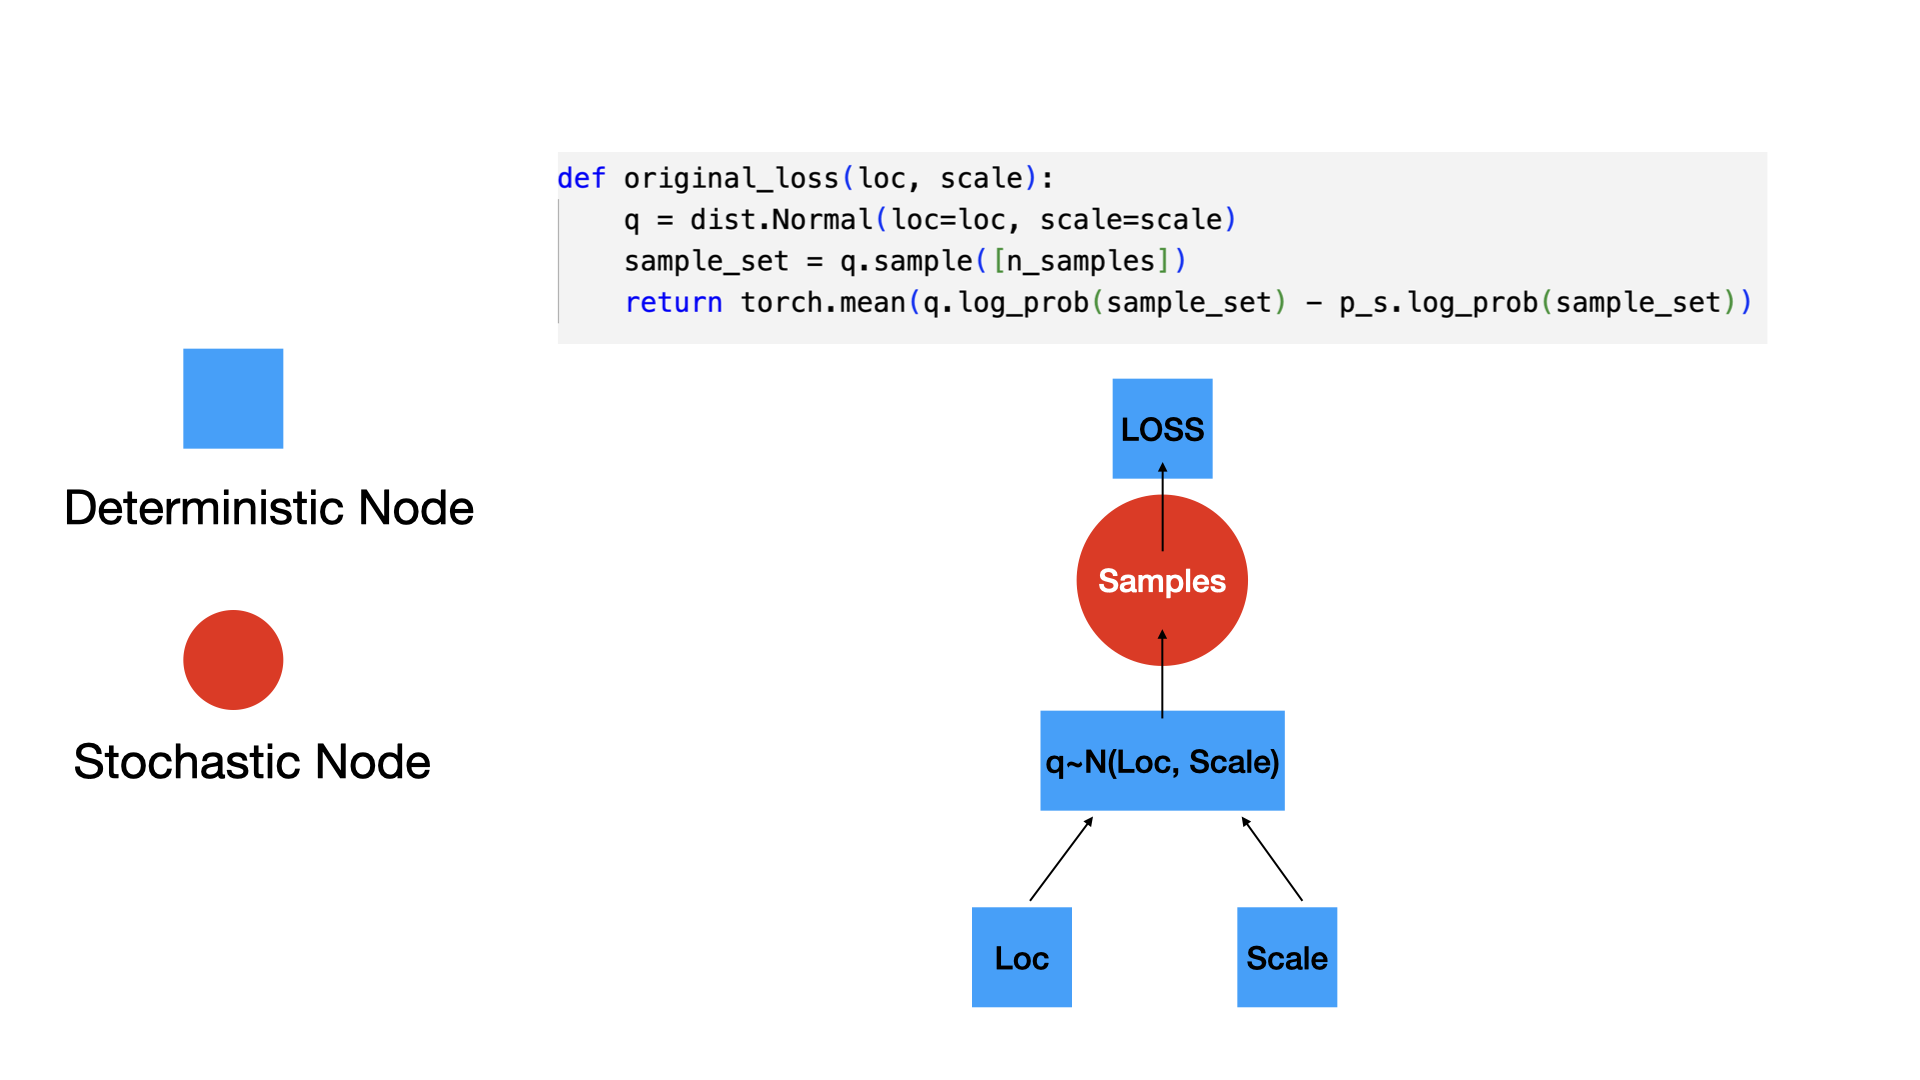
\includegraphics[width=\textwidth]{../diagrams/reparam.001.png}
    
\end{frame}

\begin{frame}{Repameterization Trick}
    New formulation (reparameterization trick)
    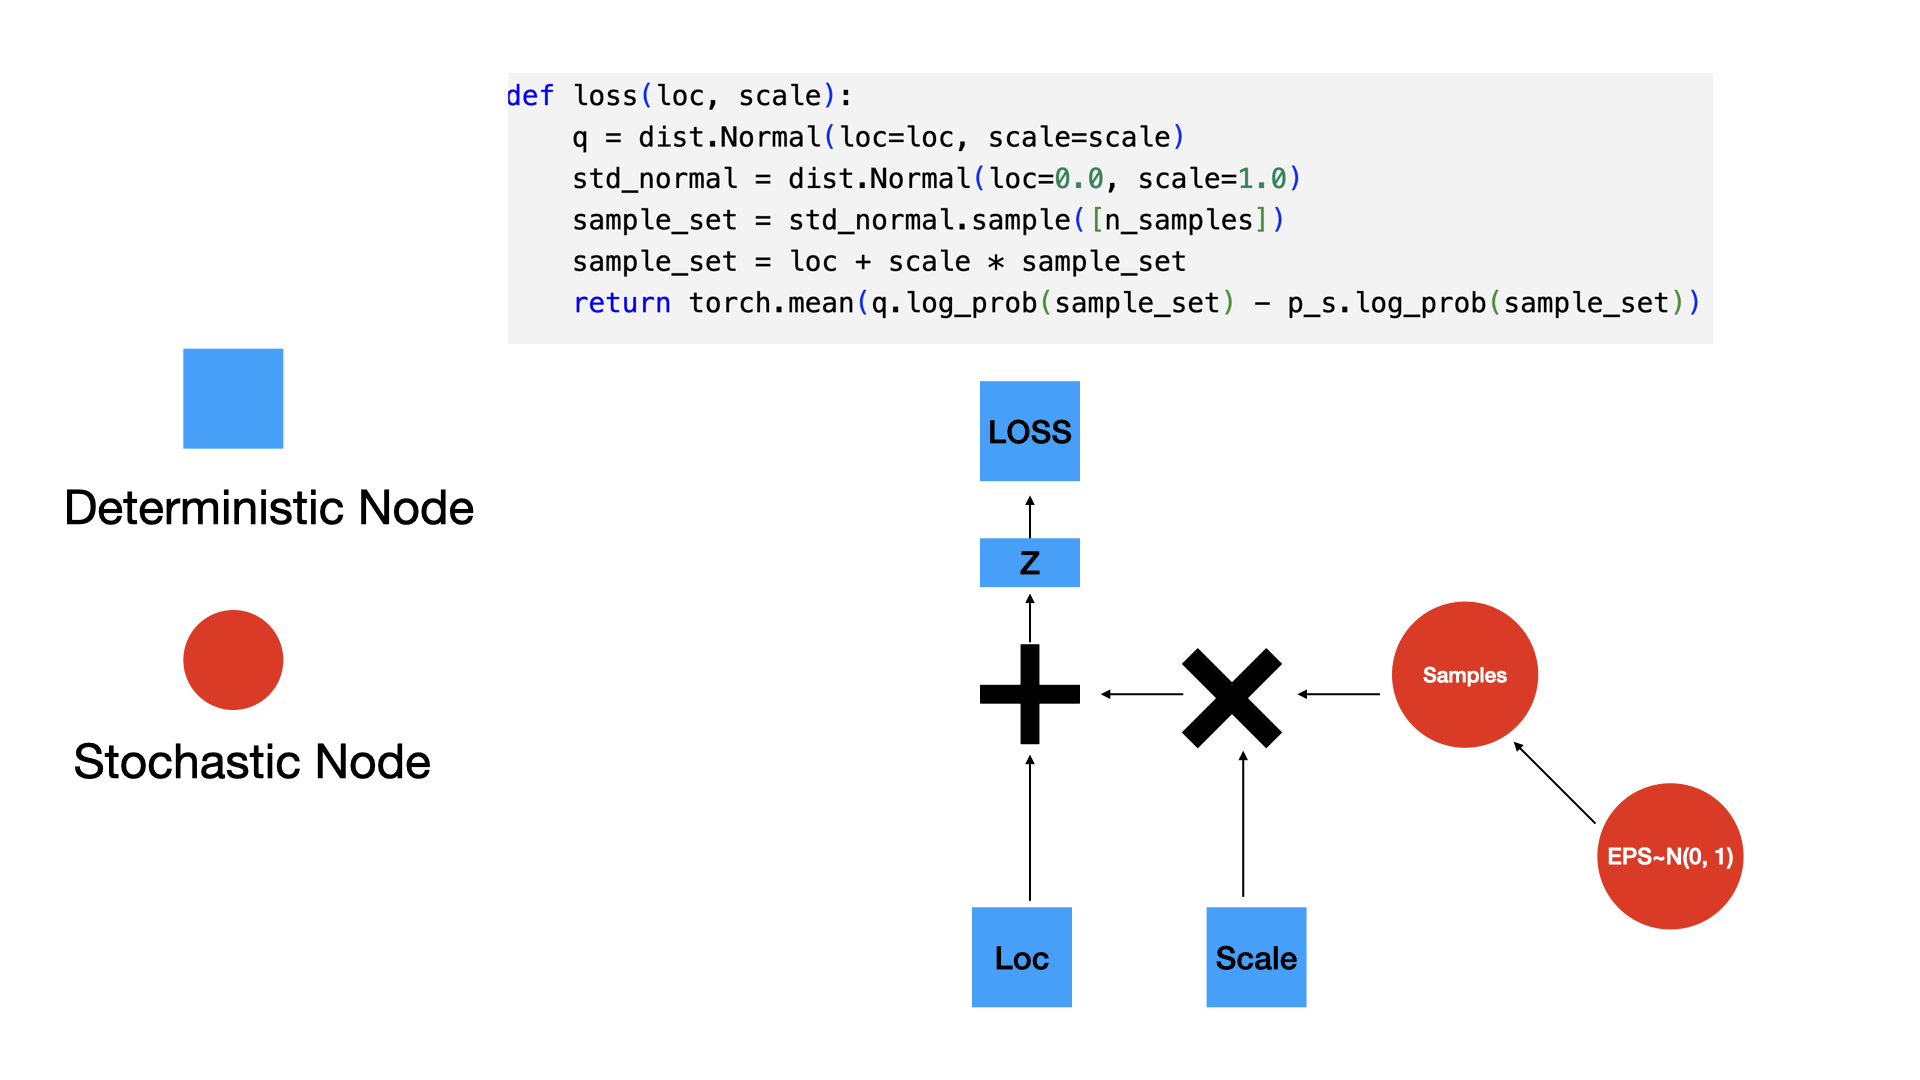
\includegraphics[width=\textwidth]{../diagrams/reparam.002.png}
    
\end{frame}

\begin{frame}
    Notebook demo
\end{frame}

\begin{frame}{Evidence Lower Bound (ELBO)}
    \begin{itemize}
        \item Our goal was to find the parameters $\psi$ of the approximating distribution $q_{\Psi}(\theta)$ such that it is as close as possible to the true posterior distribution $P(\theta|D)$.
        \item \pause $\Psi^* = \arg\min_{\Psi} \text{KL}(q_{\Psi}(\theta)||P(\theta|D))$
        \item \pause But, we do not know the true posterior distribution $P(\theta|D)$. 
        \item \pause Let us focus on the KL divergence term:
        \item \pause $\text{KL}(q_{\Psi}(\theta)||P(\theta|D)) =  \mathbb{E}_{q_{\Psi}(\theta)} \left[ \log \frac{q_{\Psi}(\theta)}{P(\theta|D)} \right]$
        \item \pause Using Bayes rule, we write: $P(\theta|D) = \frac{P(D|\theta)P(\theta)}{P(D)}$
    \end{itemize}
    
    
\end{frame}

\begin{frame}{ELBO}
    \begin{itemize}
        \item $\text{KL}(q_{\Psi}(\theta)||P(\theta|D)) =  \mathbb{E}_{q_{\Psi}(\theta)} \left[ \log \frac{q_{\Psi}(\theta)}{P(\theta|D)} \right]$
        \item Using Bayes rule, we write: $P(\theta|D) = \frac{P(D|\theta)P(\theta)}{P(D)}$
        \item \pause Substituting, we get: $\text{KL}(q_{\Psi}(\theta)||P(\theta|D)) =  \mathbb{E}_{q_{\Psi}(\theta)} \left[ \log \frac{q_{\Psi}(\theta)P(D)}{P(D|\theta)P(\theta)} \right]$
        \item \pause Expanding, we get: $\text{KL}(q_{\Psi}(\theta)||P(\theta|D)) =  \mathbb{E}_{q_{\Psi}(\theta)} \left[ \log \frac{q_{\Psi}(\theta)}{P(\theta)P(D|\theta)} + \log P(D) \right]$
        \item \pause As log-evidence, $\log P(D)$ is independent of $\Psi$, we get: $\text{KL}(q_{\Psi}(\theta)||P(\theta|D)) =  \mathbb{E}_{q_{\Psi}(\theta)} \left[ \log \frac{q_{\Psi}(\theta)}{P(\theta)P(D|\theta)} \right] + \log P(D)$
    \end{itemize}
    
\end{frame}

\begin{frame}{ELBO}
    \begin{itemize}
        \item $\text{KL}(q_{\Psi}(\theta)||P(\theta|D)) =  \mathbb{E}_{q_{\Psi}(\theta)} \left[ \log \frac{q_{\Psi}(\theta)}{P(\theta)P(D|\theta)} \right] + \log P(D)$
        \item \pause $\underbrace{\text{KL}(q_{\Psi}(\theta)||P(\theta|D))}_{\geq 0} =  \mathbb{E}_{q_{\Psi}(\theta)} \left[ \log \frac{q_{\Psi}(\theta)}{P(\theta)P(D|\theta)} \right] + \log P(D)$
        \item \pause Let us call the term $\mathbb{E}_{q_{\Psi}(\theta)} \left[ \log \frac{q_{\Psi}(\theta)}{P(\theta)P(D|\theta)} \right]$ as $\textbf{-ELBO(q)}$
        \item \pause We can see that log-evidence or $\log P(D) \geq \text{ELBO(q)}$
        \item \pause Or, we can see that the \textbf{evidence} term is lower bounded by the \textbf{ELBO} term
    \end{itemize}

    \pause 
    \begin{figure}
        \centering
        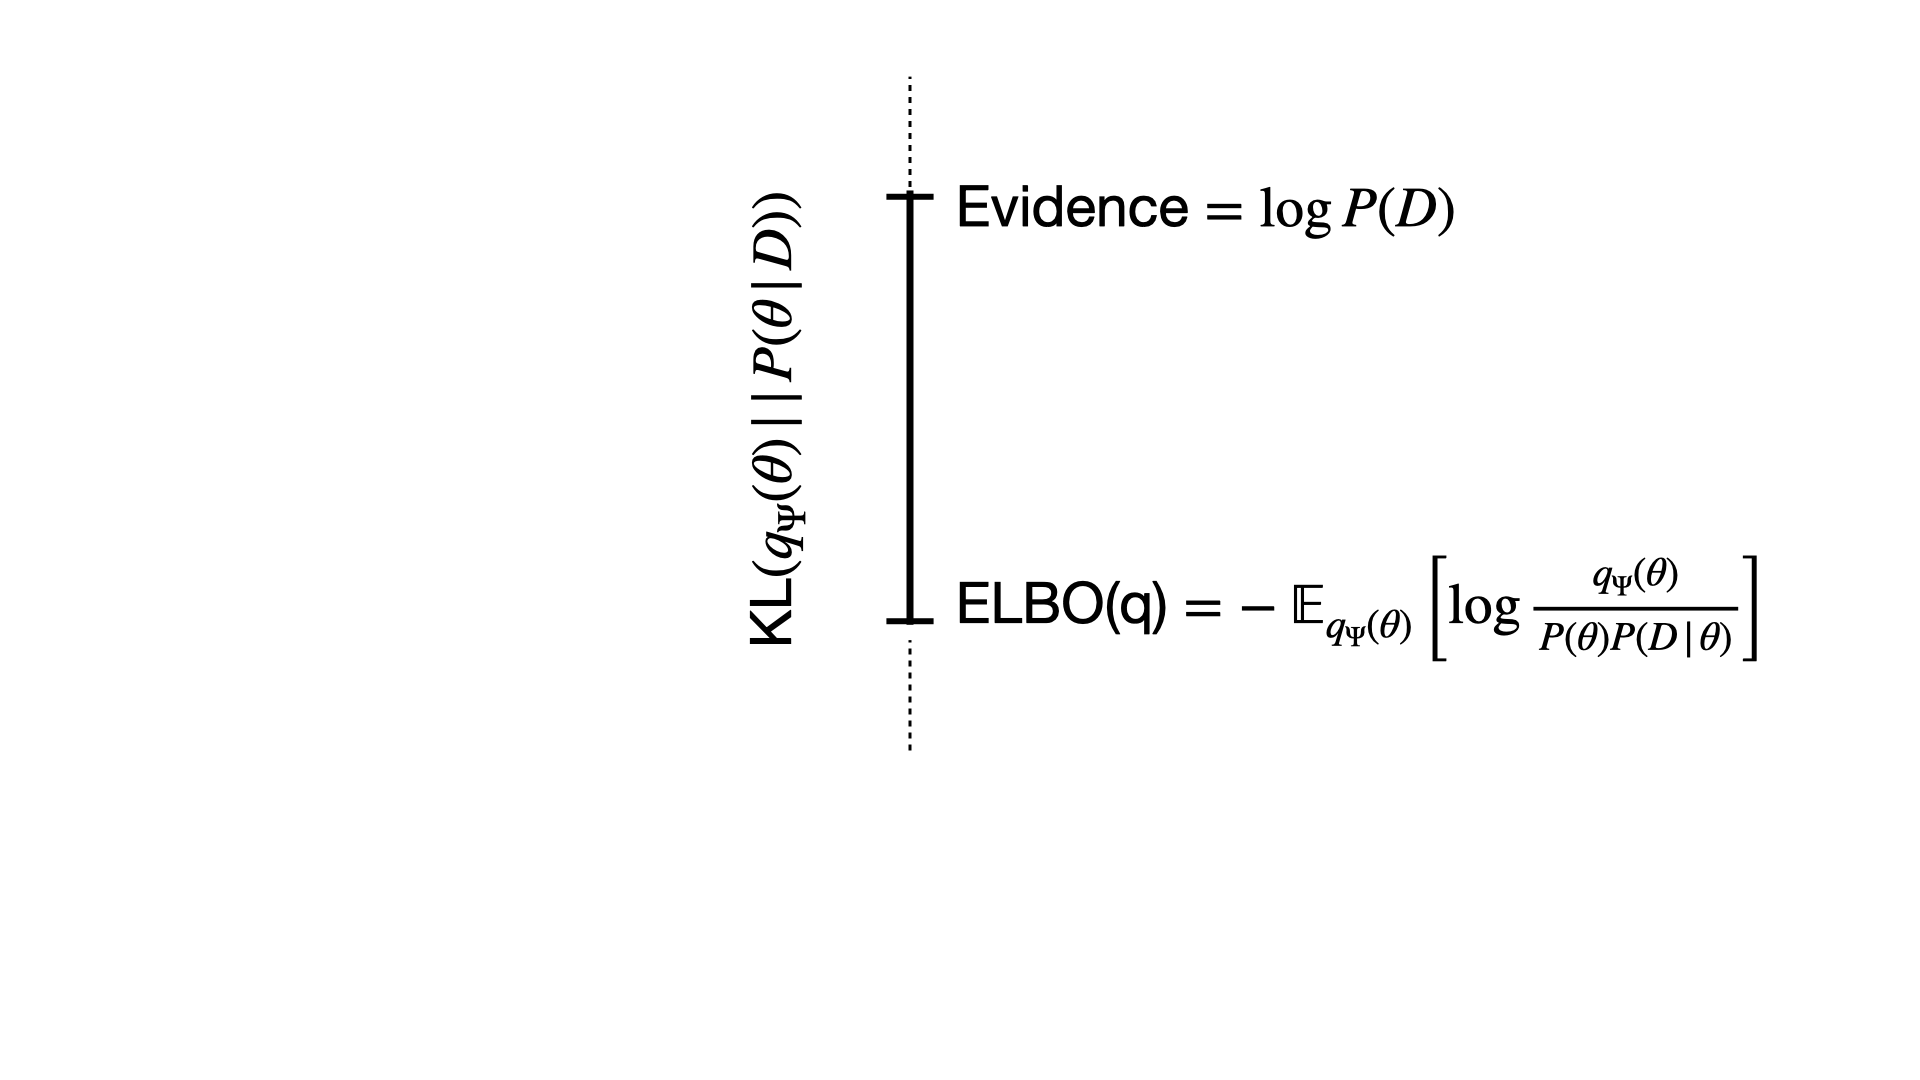
\includegraphics[width=0.5\textwidth]{../diagrams/kl-elbo.png}
        \caption{ELBO Inspired by: \url{https://mbernste.github.io/posts/elbo/}{https://mbernste.github.io/posts/elbo/})}
        \label{fig:my_label}
    \end{figure}

\end{frame}
    
\begin{frame}{Worked out example: Coin Toss}
   
\end{frame}

\begin{frame}{Worked out example: Linear Regression}
    
\end{frame}

\begin{frame}{Worked out example: Neural Networks}
\end{frame}

    


\end{document}